\section{Оборудование}
\begin{figure}[ht!]
    \center{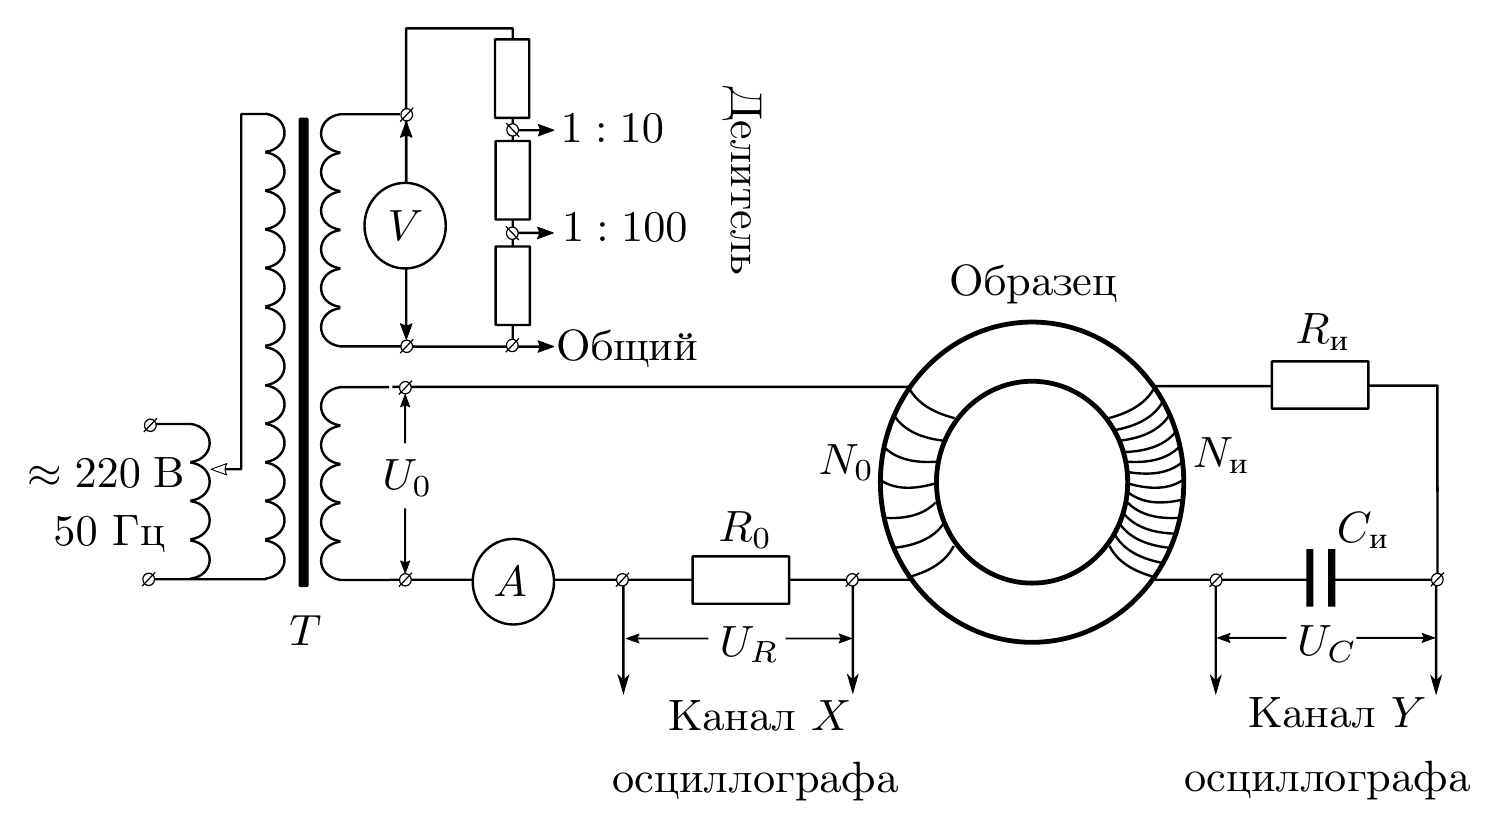
\includegraphics[width=0.8\linewidth]{../img/eq1.png}}
\end{figure}
Спомощью трансформаторного блока Т, состоящего из регулировочного автотрансформатора и разделительного понижающего трансформатора, подаётся на намагничивающую обмотку $N_{0}$  исследуемого образца.

В цепь намагничивающей катушки, на которую подаётся некоторое напряжение $U_{0}$,
последовательно включено сопротивление $R_{0}$.
Напряжение на $R_{0}$, равное $U_{R} = R_{0}I_{0}$, $I_{0}$~--- ток в намагничивающей обмотке $N_{0}$,  подаётся на канал X осциллографа. Связь напряжённости $H$ в образце и тока $I_{0}$ рассчитывается по теореме о циркуляции.
Действующее значение переменного тока в обмотке $N_{0}$ измеряется амперметром A.

Для измерения магнитной индукции $B$  с измерительной обмотки $N_{\text{и}}$ на вход RC--цепочки подаётся напряжение $U_{\text{и}}$, пропорциональное $dB/dt$. С интегрирующей ёмкости $C$  снимается напряжение $U_{C}$, пропорциональное величине $B$ и подаётся на вход Y осциллографа. Значение индукции поля $B$ рассчитывается по формуле.

Замкнутая кривая, возникающая на экране, воспроизводит в некотором масштабе (различном для осей X и Y ) петлю гистерезиса. Чтобы придать этой кривой количественный смысл, необходимо установить масштабы изображения, т. е. провести калибровку каналов X и Y осциллографа.

Калибровка канала X осциллографапроизводится с помощью амперметра A. Предварительно необходимо закоротить обмотку $N_{0}$. При закороченной
 обмотке $N_{0}$ показания эффективного тока, умноженные на $2\sqrt 2$ дадут значение удвоенной амплитуды тока, подаваемого на ось X, соответствующего ширине горизонтальной развёртки на экране.

Калибровка вертикальной оси Y , как правило, не нужна (переключатель масштабов осциллографа откалиброван при изготовлении — при условии, что ручка плавной регулировки находится в положении калибровки). Тем не менее, она может проводиться с помощью сигнала, сни маемого через делитель напряжения со второй катушки понижающеготрансформатора .
